\documentclass[a4paper,14pt]{extarticle}

\usepackage[utf8]{inputenc}

\usepackage[english,russian]{babel}

\usepackage{url}
\usepackage[unicode]{hyperref}

\usepackage{graphicx}
\addto\captionsrussian{\renewcommand{\figurename}{График}}

\usepackage[backend=bibtex,sorting=none]{biblatex}
\bibliography{bibliography}
\DefineBibliographyStrings{russian}{%
	references = {Библиография},
}

\usepackage{listings}
\lstset{captionpos=b,basicstyle=\small,tabsize=2,numbers=left}
\renewcommand\lstlistingname{Листинг}
\lstdefinelanguage{scala}{
  morekeywords={abstract,case,catch,class,def,%
    do,else,extends,false,final,finally,%
    for,if,implicit,import,match,mixin,%
    new,null,object,override,package,%
    private,protected,requires,return,sealed,%
    super,this,throw,trait,true,try,%
    type,val,var,while,with,yield},
  otherkeywords={=>,<-,<\%,<:,>:,\#,@},
  sensitive=true,
  morecomment=[l]{//},
  morecomment=[n]{/*}{*/},
  morestring=[b]",
  morestring=[b]',
  morestring=[b]"""
}

\setcounter{secnumdepth}{5}
\setcounter{tocdepth}{5}

\usepackage{geometry}
\geometry{left=3cm}
\geometry{right=2cm}
\geometry{top=2cm}
\geometry{bottom=2cm}

\linespread{1.3}

\newcommand{\todo}[1]{\textbackslash\textbackslash TODO: #1}


\begin{document}

\begin{titlepage}
\newpage

\begin{center}
Учреждение Российской Академии наук \\
Санкт-Петербургский академический университет --- \\
Научно-образовательный центр нанотехнологий РАН \\
\end{center}

\begin{flushright}
\begin{minipage}[t][12em][c]{30ex}
\begin{center}
На правах рукописи \\
\medskip
Диссертация допущена к защите \\
Зав. кафедрой \\
\hrulefill \\
<<\hspace{2em}>> \hspace{1ex} \hrulefill \hspace{1ex} 2014 г.\\
\end{center}
\end{minipage}
\end{flushright}

\begin{center}
Диссертация \\
на соискание ученой степени \\
магистра \\
\end{center}

\begin{flushleft}
Тема <<Синтаксический анализ исходного кода, содержащего инструкции препроцессора>>
\end{flushleft}

\begin{flushleft}
Направление: 010600.68 --- Прикладные математика и физика
\end{flushleft}

\begin{flushleft}
Магистерская программа: <<Математические и информационные технологии>>
\end{flushleft}

\begin{flushleft}
Выполнил студент \hfill C.A. Савенко
\end{flushleft}

\begin{flushleft}
Руководитель: \hfill С.С. Игнатов
\end{flushleft}

\begin{flushleft}
Рецензент: \\
к.ф.-м.н., доцент \hfill Д.Ю. Булычев
\end{flushleft}

\vspace{\fill}

\begin{center}
Санкт-Петербург \\
2014 г. \\
\end{center}

\end{titlepage}


\tableofcontents

\clearpage
\section{Введение}

Для создания многих средств для работы с исходным кодом - таких, как браузеры исходного кода, инструменты автоматического поиска ошибок, среды разработки, компиляторы требуется разработать синтаксический анализатор - инструмент, позволяющий сопоставить входной текст с грамматикой языка с тем, чтобы получить дерево синтаксического разбора\cite{aho}.

Задача разработки синтаксических анализаторов (парсеров) на сегодняшний день решается одним из следующих способов:
\begin{itemize}
	\item написание парсера вручную;
	\item использование средств автоматической генерации синтаксическх анализаторов таких, например, как ANTLR\footnote{\url{http://www.antlr.org/}}, Bison\footnote{\url{http://www.gnu.org/software/bison/}}, JavaCC\footnote{\url{https://javacc.java.net/}};
\end{itemize}
Использование парсер-генераторов позволяет существенно снизить трудозатраты при разработке инструментов обработки естественных и искуственных языков.

Часто при разработке программных продуктов в исходный код на языке программирования добавляются инструкции препроцессора, позволяющие повысить выразительность используемого языка программирования посредством текстовых подстановок из других файлов, осуществения макроподстановок, использования условной компиляции. Непрепроцессированный код также может зависеть от переменных окружения, переданных препроцессору, - тогда в одном файле с исходным кодом может быть описано сразу несколько различных программ. Это используется для создания целых семейств программных продуктов с общей кодовой базой\cite{flightsoftwareproductline}, а также для создания высоко конфигурируемых программных систем. Использование текстовых препроцессоров при разработке программного обеспечения не является экзотикой - в некоторых языках, например C, C++, C\#, препроцессирование исходного кода является одним из этапов компиляции.

Применение препроцессора приводит и к появлению ошибок, проявляющихся только при компиляции в некоторых конкретных конфигурациях --- это могут быть синтаксические ошибки, ошибки типизации, ошибки при разрешении зависимостей и многие другие типы ошибок. Это приводит к необходимости обработки инструкций препроцессора в инструментах анализа исходного кода.

Для разработки таких инструментов требуются синтаксические анализаторы, способные обрабатывать "смесь" из инструкций препроцессора и конструкций целевого языка программирования. Таким парсерам необходимо обрабатывать случаи "прерывания" грамматических конструкций языка инструкциями препроцессора, производить макроподстановки, обрабатывать варианты программы, которые могут быть получены при различных конфигурациях препроцессора.

Синтаксические анализаторы для языка С, обладающие описанной функциональностью, описаны в работах \cite{superc} и \cite{typechef}. В данной работе представлен инструмент для упрощения разработки таких синтаксических анализаторов. 

\clearpage

\section{Постановка и анализ задачи}

Проблема синтаксического разбора непрепроцессированного кода поднимается в различных публикациях уже достаточно продолжительное время. Это связано в первую очередь с большой популярностью языка С и, соответственно, его препроцессора - cpp. Далее будет описана основная функциональность препроцессора cpp и подходы к анализу непрепроцессированного кода.

\subsection{Описание функциональности препроцессора}

Препроцессор cpp предоставляет следующую функциональность: включение файлов с исходным кодом (посредством директив \#include), объявление и использование макроопределений (\#define), условная компиляция основанная на статических условиях (директивы \#if, \#ifdef, \#ifndef, и т. д.).

\todo{добавь сюда пример кода на С с условной компиляцией}

Как видно из примера, \todo{что-то типа "в зависимости от того объявлено ли макроопределение ..."}, результатом обработки исходного кода препроцессором могут быть два различных варианта программы. Набор предзаданных макроопределений позволяет выбрать единственный вариант программы на языке С, который впоследствии подаётся на вход транслятору. Далее такой набор определений будем называть конфигурацией препроцессора.

Ясно, что программист, редактируя исходный код с инструкциями препроцессора, может производить изменения одновременно в огромном количестве программ, получаемых в различных конфигурациях, что зачастую приводит к ошибкам\cite{ribeiro}. Обнаружение ошибок и другие задачи, связанные с обработкой непрепроцессированного исходного кода требуют рассмотрения сразу нескольких возможных конфигураций препроцессора.

\subsection{Обзор способов разбора непрепроцессированного кода}

Существует несколько подходов к анализу непрепроцессированного кода с учётом конфигураций препроцессора.

\begin{enumerate}

\item 

Обработка конфигураций "по одной". Идея подхода в том, чтобы производить поиск ошибок и решать другие задачи обработки исходного кода в каждой конфигурации препроцессора по отдельности. Подход очень прост в реализации, он применяется как неявно - при сборке проектов с разными конфигурациями, так и явно - например, в средах разработки Xcode\footnote{\url{https://developer.apple.com/xcode/}} и KDevelop\footnote{\url{http://kdevelop.org/}}.

Однако, использование этого подхода позволяет охватывать проекты целиком, так как большие проекты содержат огромное количество конфигураций. Например, сборка ядра Linux\footnote{\url{https://www.kernel.org/}} требует установки значений более 10000 макроопределений\cite{typechef}, что исключает возможность использования такого подхода для исчерпывающего анализа кода.

\item

Применение эвристик, основанных на типичных случаях использования препроцессора. Подход состоит в том, чтобы частично интерпретировать инструкции препроцессора, получая некоторое представление исходного кода с информацией о его вариантах в разных конфигурациях. Использование такого метода не позволяет обрабатывать код полностью, так как обработка всех возможных вариантов взаимодействия инструкций препроцессора с конструкциями языка программирования не представляется возможной.

Тем не менее, этот подход позволяет достичь удовлетворительных результатов в некоторых задачах. Так, например, в Eclipse CDT\footnote{\url{http://www.eclipse.org/cdt/}} --- интегрированной среде разработки для языков С и С++ --- реализована подсветка синтаксиса и рефакторинги, учитывающие некоторые случаи использования препроцессора.

\item

Построение графа, содержащего исходный код для всех возможных конфигураций препроцессора. Идея этого метода состоит в том, чтобы неявно построить абстрактные синтаксические деревья для всех возможных конфигураций препроцессора. Таким неявным представлением является направленный ациклический граф, в котором каждой возможной конфигурации препроцессора соответствует некоторый путь из истока в сток. Подобные структуры данных применяются для хранения результатов синтаксического анализа текстов на языках, содержащих неоднозначности\cite{parseforests}.

\end{enumerate}

Несмотря на очевидные преимущества третьего подхода над первыми двумя, он очень редко применяется на практике. Отчасти это связано с высокой трудоёмкостью его реализации.

\subsection{Цель работы}

При рассмотрении существующих подходов к задаче синтаксического анализа исходного кода, содержащего инструкции препроцессора, выяснилось, что подходы, приводящие к хорошим результатам, используют лишь знание о синтаксисе языка препроцессора, семантике инструкций препроцессора и синтаксисе языка программирования в том или ином виде.

Это наблюдение привело к предположению о возможности создания инструмента, позволяющего производить синтаксический анализ исходного кода, содержащего инструкции препроцессора, используя парсер, либо грамматику языка программирования, парсера препроцессора и некоторого интерпретатора его инструкций.

Целью настоящей работы является создание такого инструмента.

\subsection{Задачи работы}

Для достижения поставленной цели необходимо решить следующие задачи:

\begin{itemize}

\item изучить существующие решения задачи синтаксического разбора непрепроцессированного кода;

\item разработать алгоритм, позволяющий использовать готовый синтаксический анализатор, либо грамматику языка программирования, для синтаксического анализа исходного кода, содержащего инструкции препроцессора;

\item реализовать разработанный алгоритм;

\item реализовать синтаксический анализатор для языка Erlang с инструкциями препроцессора, использующий разработанный алгоритм.

\end{itemize}





\clearpage

\section{Существующие решения}

Этот раздел содержит подробности реализаций подхода к решению проблемы синтаксического анализа непрепроцессированного исходного кода, состоящего в построении графа, содержащего деревья синтаксического разбора для всеx конфигураций препроцессора (см. описание подхода в подразделе \ref{subsec:unpreprocessed_parsing_methods}).

Наиболее известными реализациями этого подхода являются SuperC\cite{superc} и TypeChef\cite{typechef}.

\subsection{Общие идеи}
\label{subsec:commonideas}

Построение графа, содержащего деревья синтаксического разбора для всех конфигураций препроцессора, так или иначе включает в себя два этапа:

\begin{enumerate}

\item Частичное препроцессирование или лексический анализ, сохраняющий конфигурацию.

Выполняется интерпретация инструкций препроцессора, с сохранением информации об условных ветвлениях, и лексический анализ;
\item Синтаксический анализ, сохраняющий конфигурацию.

Используется результат выполнения предыдущего этапа для построения графа разбора, содержащего синтаксические деревья для всех конфигураций препроцессора;

\end{enumerate} 

\subsubsection{Лексический анализ, сохраняющий конфигурацию}
\label{subsubsec:configurationpreservinglexing}

Работа, выполняемая на этом этапе, условно состоит из двух частей --- интерпретации инструкций препроцессора и проведения лексического анализа входного текста. Условность здесь состоит в том, что эти части могут выполняться одновременно, если языком препроцессора используются те же лексемы, что и языком программирования.

Инструкции препроцессора интерпретируются аналогично тому, как это делает сам препроцессор, за тем исключением, что строятся варианты выходных последовательностей одновременно для всех конфигураций. Более подробно работа лексического анализатора, сохраняющего конфигурацию описана в подразделе \ref{lexingandpreprocessing} на примере его реализации в проекте SuperC.

Результатом выполнения этого этапа является последовательность лексем и узлов условного ветвления, представленная в том или ином виде. Узлы ветвления представляют собой наборы из подпоследовательностей лексем и узлов условного ветвления, предваренных так называемыми условиями наличия (presence conditions). Каждый такой набор внутри узла ветвления соответствует некоторой альтернативной ветви условной компиляции в исходном непрепроцессированном коде.

\subsubsection{Синтаксический анализ, сохраняющий конфигурацию}

Этот этап состоит в преобразовании входной последовательности из лексем и узлов условного ветвления в абстрактное синтаксическое дерево (либо абстрактный синтаксический лес), содержащий вершины, соответствующие конструкциям языка программирования, как в обыкновенном абстрактном синтаксическом дереве, а также вершины условного ветвления, каждая ветвь которых соответствует некоторой альтернативной ветви условной компиляции.

Появление узла ветвления во входной последовательности лексем может приводить к различной интерпретации лексем и уже разобранных конструкций, предшествующих текущей позиции. Это может привнести существенные сложности при разборе альтернативных ветвей условной компиляции. Так, в листинге \ref{lexemeinterpretation} выражение справа от знака присваивания может быть либо числовой константой, либо аддитивным выражением. Это потребует переноса места ветвления в позицию следующую за символом равенства.

\begin{minipage}{\linewidth}
\begin{lstlisting}[caption={Пример различной интерпретации лексем, предшестующих блоку условной компиляции},label=lexemeinterpretation,language=C]
int main(int argc, char ** argv) {
	int x = 0
#ifdef RET_1
	+ 1	
#endif
	;
	return x;	
}
\end{lstlisting}
\end{minipage}

Помимо проблемы выбора места ветвления, имеет место проблема выбора места слияния. Она состоит в том, что лексемы, следующие за узлом условного ветвления могут быть проинтерпретированы по-разному для каждой из альтернативных ветвей.

Слишком раннее ветвление, равно как и слишком позднее слияние могут привести к многократному разбору одних и тех же участков кода, что приводит к существенному снижению производительности и увеличению объёма используемой памяти.

\todo{Добавить пример удачного и неудачного слияния. Можно сослаться, например на "дисциплинированные" формы в ранних версиях TypeChef}

\subsection{Синтаксический анализ непрепроцессированного кода на языке С}

На языке программирования С с момента его создания было написано огромное количество программного обеспечения различной сложности --- в том числе и наиболее сложные программные системы: ядра операционных систем, системы управления базами данных, и т. д.. В связи с этим имеется большой спрос на средства работы с исходным кодом на языке С --- браузеры кода, средства автоматического поиска ошибок, инструменты для рефакторинга, что, в свою очередь, пробудило интерес исследователей к проблеме синтаксического анализа непрепроцессированного кода на языке С.

\subsubsection{SuperC}

Проект SuperC является частью проекта xtc\footnote{eXTensible Compiler --- \url{http://cs.nyu.edu/rgrimm/xtc/}} Нью-Йоркского Университета. В этом проекте успешно решается проблема синтаксического анализа кода на языке С с инструкциями препроцессора, что подтверждается успешным разбором кода ядра Linux для архитектуры x86.

SuperC использует описанный в подразделе \ref{subsec:commonideas} двухэтапный подход. Рассмотрим более подробно каким образом реализованы эти этапы.

\paragraph{Лексирование и препроцессинг}
\label{lexingandpreprocessing}

Для того, чтобы сформировать единицу компиляции, препроцессору, сохраняющему конфигурацию необходимо обработать следующие инструкции препроцессора: объявления и удаления макроопределений, директивы включения файлов, вызовы макроопределений.

Для корректной обработки этих инструкций, препроцессору, среди прочего, необходимо производить разрешение имён макроопредлений. Это решается при помощи поддержания таблицы макроопределений на протяжениип обработки входных файлов. В эту таблицу вносятся записи, соответствующие директивам препроцессора \#define и \#undef. При этом объявления равно как и удаления макроопределений могут появляться в различных ветвях статических условных блоков, что приводит к тому, что, в зависимости от конфигурации один и тот же вызов макроопределения может быть проинтерпретирован совершенно по-разному - возможны не только различные варианты макроподстановок, но и сами вызовы. Поэтому записи в таблице макроопределений ассоциируются с условиями их наличия, используемыми впоследствии для разрешения имён в различных ветвях условной компиляции.

\autoref{macrocalls} иллюстрирует некоторые случаи различных вызовов и подстановок макроопределений. Так, в случае наличия в конфигурации препроцессора объявления OP\_FUN, в двенадцатой строке будет произведена подстановка макроопределения без аргументов. Eсли же OP\_FUN окажется необъявленным, но будет объявлен OP\_ID - будет произведена подстановка макроопределения с одним аргументом. В случае, если оба этих объявления не будут присутствовать, лексема, соответствующая имени макроопределения должна быть пропущена, а лексемы, соответствующие возможным аргументам вызова, проанализированы на предмет наличия других вызовов макроопределений.

\begin{minipage}{\linewidth}
\begin{lstlisting}[caption={Различные вызовы макроопределения при различных конфигурациях препроцессора},language=C,label=macrocalls]
#ifdef OP_FUN
int __op_fun(int x) {
	return x + 2;
}
#define OP __op_fun
#elif OP_ID
#define OP(X) X
#endif

int main(int argc, char ** argv) {
	int x = 0;
	x = OP(x);
	return x;	
}
\end{lstlisting}
\end{minipage}

Таким образом, различные варианты подстановки для одного и того же вызова макроопределения, равно как и различные вызовы макроопределений, полученные из тех же лексем, порождают неявные блоки условной компиляции, которые должны быть обработаны как препроцессирующим лексером, так и парсером на следующем этапе точно таким же образом, как и явные блоки условной компиляции, заданные при помощи директив препроцессора \#if, \#ifdef, \#ifndef и др..

Вызовы макроопределений могут также пересекать границы блоков условной компиляции \todo{нужно пример?}, что приводит к необходимости специальной обработки таких ситуаций, состоящей в дубликации лексем, составляющих вызов макроопределения.

Как уже было сказано ранее, для корректной обработки статических условий необходимо поддерживать условия наличия тех или иных участков кода. При этом трансформация статических условий в условия наличия зачастую требует частичного вычисления булевых выражений. Разработчики SuperC используют в своём решении двоичные диаграммы принятия решений\footnote{Binary Decision Diagrams (BDD) --- \url{http://en.wikipedia.org/wiki/Binary\_decision\_diagram}}, а именно - библиотеку JavaBDD\footnote{\url{http://javabdd.sourceforge.net/}}. Это позволяет эффективно сравнивать условия наличия, а также выявлять недостижимые ветви условной компиляции. \todo{Нужно описать как именно транслируются статические условия в BDD?}

Результатом работы препроцессирующего лексера является направленный ациклический граф, состоящий из лексем с условиями их присутствия. В SuperC этот граф представлен последовательностью лексем языка с дополнительными лексемами, обозначающими точки ветвления и границы ветвей условной компиляции.

\paragraph{Синтаксический анализ}

Парсер, применяемый в проекте SuperC, основывается на LR-анализаторе (см. \cite{aho}), генерируемом парсер-генератором Bison\footnote{\url{http://www.gnu.org/software/bison/}}.

Работа LR-анализаторов строится на основе стека, содеражащего терминальные и нетерминальные символы грамматики. Каждый шаг алгоритма LR-анализатора представляет собой одно из 4х возможных действий: сдвиг - помещение лексемы из входного буффера на стек, редукция - замена нетерминалом одного или нескольких верхних элементов стека, принятие - успешное завершение парсинга, отвержение - завершение парсинга с ошибкой. Действие выбирается в зависимости от входной лексемы и текущего состояния стека.

Разработчики SuperC аргументируют выбор именно LR-анализатора в качестве основы для парсера сохраняющего конфигурацию следующими пунктами:

\begin{itemize}
\item Возможность использования LR парсер-генераторов для создания LR-таблиц, что значительно упрощает разработку;
\item Удобство использования состояния парсера для обработки ветвей условной компиляции: достаточно использовать персистентный стек, реализованный на основе односвязного списка;
\item Поддержка LR-парсерами широкого класса языков программирования.
\end{itemize}

Сам же FMLR-анализатор (Fork Merge LR parser) представляет собой алгоритм похожий по структуре на планировщик задач, где задачами выступают LR-подпарсеры. Алгоритм поддерживает очередь парсеров с соответствующими им условиями наличия и состояниями чтения входного буфера.

На каждом шаге алгоритма из очереди вынимается один парсер, для которого, в зависимости от следующего символа и состояния парсера выполняется одно из следующих действий:

\begin{itemize}
\item LR-действие, выбранное подпарсером и помещение подпарсера в конец очереди;
\item Создание подпарсеров этого подпарсера для каждой из следующих возможных лексем, помещение этих подпарсеров в конец очереди.
\end{itemize}

После выполнения действия очередь парсеров исследуется на возможность слияния нескольких подпарсеров в один - это возможно лишь в том случае, если парсеры находятся на одном и том же месте во входном буфере и их LR-стеки совпадают. 

Помимо этого SuperC ограничивает множество возможных точек слияния определенным набором редукций исходной грамматики - этот набор задаётся вручную. Если такие подмножества парсеров находятся, то каждое подмножество заменяется одним подпарсером с условием наличия выраженным как логическое ИЛИ условий наличия объединенных парсеров.

\subsubsection{TypeChef}

TypeChef - исследовательский проект, объединивший усилия исследователей из многих университетов, имеющий своей целью поиск ошибок, вызванных интенсивным использованием препроцессора, в программах на языке С.

В основе алгоритма разбора непрепроцессированного исходного кода  так же, как и в случае SuperC, лежит двухэтапный подход, поэтому далее будут описаны только особенности, отличающие TypeChef от SuperC.

\paragraph{Лексирование и препроцессинг}

Логика работы лексирующего препроцессора, сохраняющего конфигурацию, реализованного в TypeChef идентична реализации SuperC за тем исключением, что для работы с условными выражениями используются пропозициональные формулы в конъюнктивной нормальной форме, для которых решается задача выполнимости\footnote{SAT --- \url{http://en.wikipedia.org/wiki/Boolean\_satisfiability\_problem}}, вместо двоичных диаграмм принятия решений. 

\paragraph{Синтаксический анализ}

Синтаксический анализатор TypeChef основан на расширении библиотеки парсер-комбинаторов языка Scala. Это расширение представляет собой набор парсер-комбинаторов, позволяющих описывать точки возможных условных ветвлений и слияний парсеров. Более подробно о реализации этого расширения можно прочесть в \cite{typechef2}.


\subsection{Возможности адаптации решений к другим языкам}
\label{subsec:solutionsadaptation}

Не смотря на то, что изученные проекты TypeChef и SuperC были изначально нацелены на синтаксический анализ языка С с инструкциями препроцессора cpp, они предоставляют возможности для распространения используемых подходов на другие языки. Однако, имеются препятствия к такому их использованию.

\subsubsection{TypeChef}

Для того, чтобы использовать TypeChef для синтаксического анализа кода на языке отличном от С, требуется описать целевой язык, используя библиотеку парсер-комбинаторов Scala с расширениями, предоставляемыми TypeChef.

Описание целевого языка при помощи парсер-комбинаторов вызвать некоторые проблемы, связанные, например, c использованием леворекурсивных правил в грамматике. 

Помимо этого, понадобится воспользоваться семью парсер-комбинаторами, описывающими возможные места ветвлений и слияний, что требует хорошего представления о принципах работы TypeChef.

\subsubsection{SuperC}

Серьёзных усилий требует и SuperC. Для реализации синтаксического анализатора языка программирования с инструкциями препроцессора, SuperC требует от разработчика следующее:

\begin{itemize}
\item Описание лексера со специальными аннотациями, указывающими какие лексемы являются запятыми, скобками, решёткой, двойной решёткой (эти лексемы используются препроцессором языка С);
\item Описание грамматики языка для парсер-генератора Bison;
\item Аннотации к правилам грамматики, указывающих является ли левая часть этого правила завершенной семантической единицей (это используется при создании условных узлов для разных ветвей статических условий);
\item Реализация семантических действий при разборе той или иной синтаксической конструкции - например, построение узлов AST.
\end{itemize}

Дополнительно разрабочик может самостоятельно реализовать логику ветвления и слияния подпарсеров, что предоставляет интересные возможности для построения графов синтаксического разбора именно в той форме, в которой их хочет видеть разработчик.

Хочется заметить, что это достаточно большой объём работы, которая требует не только квалификации разработчика в области LR анализаторов, но и хорошей степени знакомства с проектом SuperC.

\clearpage

\section{Синтаксический анализ непрепроцессированного кода}

В этом разделе описывается алгоритм, позволяющий производить синтаксический анализ исходного кода, представленного в виде графа лексем и точек ветвлений (см. подраздел \ref{subsubsec:configurationpreservinglexing}).

\subsection{Мотивация}

Для построения графа синтаксического разбора, содержащего деревья разбора для всех возможных конфигураций препроцессора, необходимо знание о структуре языка, либо о синтаксическом анализаторе, используемом для разбора языка программирования.

В проектах SuperC и TypeChef использовалось знание о синтаксических анализаторах. А именно, SuperC использует LR-действия синтаксического анализатора языка программирования в явном виде, TypeChef же предлагает использовать свои инструменты для создания синтаксического анализатора языка программирования. Первое решение основывается на LR-анализаторах, второе - на LL, - и в первом и во втором случае может потребоваться модификация грамматики языка программирования, с тем, чтобы удовлетворить ограничения на обрабатываемые языки, накладываемые этими классакми парсеров.

Результатом такого выбора стала высокая трудоёмкость адаптации этих решений для работы с другими языками программирования (см. подраздел \ref{subsec:solutionsadaptation}).

Поэтому к алгоритму синтаксического анализа непрепроцессированного кода, разрабатываемому в настоящей работе, предъявляются следующие требования:

\begin{itemize}
\item Использование только грамматики языка программирования;
\item Возможность синтаксического анализа исходного кода на любых языках, описываемых контекстно-свободными грамматиками \cite{cfg}.
\end{itemize}

Для удовлетворения данных требований был разработан универсальный алгоритм синтаксического анализа, основанный на алгоритме Earley \cite{earley68}.

\subsection{Алгоритм Earley}
Алгоритм синтаксического анализа Earley напрямую использует грамматику языка программирования и позволяет производить разбор текстов на языках, содержащих неоднозначности.

Результатом работы алгоритма является последовательность состояний, по которой можно определить принадлежность входного текста языку, а также восстановить все возможные деревья разбора. Далее будет описан сам алгоритм.

Как уже было замечено ранее, алгоритм строит последовательность некоторых состояний. Каждое состояние соответствует входной лексеме, для которой это состояние было получено и представляет собой упорядоченное множество элементов Earley (Earley item). Элемент Earley представляет собой продукцию грамматики с индексом в ней, обозначающимся точкой. Например, $A \to \cdot B$, $A \to B \cdot $, $A \to x \cdot B$. Часть продукции слева от точки - уже совпала со входом, а часть справа соответствует ожидаемому входу. Кроме этого, в элементе Earley сохраняется номер состояния первого появления этого элемента.

На каждом шаге алгоритм заполняет текущее состояние и инициирует следующее. Первое состояние алгоритма инициализируется элементами Earley, соответствующими начальному символу грамматики с точкой перед телом продукции. Рассмотрим теперь каким образом завершается состояние $n$ и инициируется состояние $n+1$. Производятся три операции:

\begin{itemize}

\item Предсказание. Для каждого элемента Earley из состояния $n$, имеющего нетерминал после точки, в состояние $n$ добавляются элементы Earley, соответствующие всем продукциям грамматики для этого нетерминала, с точками перед телами продукций.

\item Сканирование. Для каждого элемента Earley из состояния $n$, имеющего терминал после точки, совпадающий с входной лексемой на этом шаге, в состояние $n+1$ добавляется элемент Earley, с точкой сдвинутой за поглощенный терминал.

\item Завершение. Эта операция производится для каждого элемента Earley из состояния $n+1$, в котором точка находится после тела продукции, - это соответствует окончанию сопоставления продукции тексту. Если элемент Earley соответствует продукции для некоторого нетерминала $A$, то производится поиск продукций, имеющих точку перед этим нетерминалом в состоянии, соответствующем первому появлению текущего элемента. В состояние $n+1$ добавляются элементы Earley, соответствующие поглощенному нетерминалу $A$.

\end{itemize}

В листинге \ref{earleyrecognizer} приведена функция doEarleyStep, в которой производятся описанные выше действия.

\begin{minipage}{\linewidth}
\begin{lstlisting}[caption={Псевдокод шага алгоритма Earley},language=Scala,label=earleyrecognizer]
def doEarleyStep(lexeme, chart) = {
	val currentCol = chart.lastColumn
	val nextCol = chart.newColumnt
	predict(currentCol)
	scan(lexeme, currentCol, nextCol)
	complete(nextCol)
}

def predict(currentCol) = 
	currentCol.items.forEach(predictForItem(_, currentCol))

def predictForItem(item, currentColumn) = {
	if (item.isComplete || item.nextSymbol.isTerminal) return
	val productions = Grammar .productionsFor(item.nextSymbol)
	productions.forEach(production => {
		val item = currentColumn.addItem(production)
		if (item != null) predictForItem(item)
	})
}

def scan(lexeme, currentCol, nextCol) = 
	currentCol.items.filter(_.expects(lexeme))
		.forEach(nextCol.addItem(_.consume(lexeme)))
	
def complete(nextCol) = 
	nextCol.items.forEach(completeForItem(_, nextCol))

def completeForItem(item, nextCol) = {
	if (!item.isComplete) return
	item.startColumn.items.filter(_.expects(item))
		.forEach(startColItem => {
			val newItem = nextCol.addItem(startColItem.consume(item))
			if (newItem != null)
				completeForItem(newItem, nextCol)		
		})
}
\end{lstlisting}
\end{minipage}

Так, результатом работы алгоритма станет последовательность из $N+1$ состояния для входного текста длины $N$ лексем. Если входной текст принадлежит языку, грамматика которого использовалась для разбора, то в последнем состоянии будет находиться хотя бы один завершенный элемент Earley, впервые добавленный в первом состоянии, соответствующий начальному символу грамматики.

Описанный выше алгоритм производит только распознавание входа, т. е. позволяет определить принадлежит ли входной текст языку, описываемому используемой грамматикой. Несколько модифицировав алгоритм распознавания, можно получить средство для восстановления деревьев разбора.

Для этого необходимо при выполнении сканирования и завершения сохранять указатели/ссылки на элементы Earley, из которых мог быть получен новый элемент Earley (это может быть реализовано в функции consume, используемой в листинге \ref{earleyrecognizer}). 

Обратный проход по этим указателям, начиная с состояния, соответствующего завершенному разбору для начального символа, будет соответствовать одному из возможных деревьев разбора. Более подробно о преобразовании алгоритма распознавания в парсер можно прочесть в оригинальной работе \cite{earley68}, а также в \cite{recognizertoparser}.

Замечательная особенность алгоритма состоит в том, что он работает с любой контекстно-свободной грамматикой и не требует её приведения к какому-либо специальному виду.

\subsection{Модификация алгоритма Earley}
\label{subsec:earleymodification}

Основная идея алгоритма состоит в том, чтобы для различных ветвей условной компиляции строить различные последовательности состояний, сохраняя условия наличия, после чего объединять полученные наборы состояний.

Далее описывается модификация алгоритма Earley, позволяющая работать с графом, полученным на выходе препроцессирующего лексера, сохраняющего конфигурацию, a также необходимые модификации алгоритма восстановления графа разбора.. 

\subsubsection{Распознавание}

Алгоритм начинает свою работу точно как оригинальный алгоритм распознавания Earley.

Если в процессе работы встречается точка ветвления в графе лексем, то создаются новые распознаватели Earley для каждой из ветвей условной компиляции. В каждой ветви используется состояние, соответствующее состоянию перед точкой ветвления, в качестве начального. Далее этот же алгоритм рекурсивно обрабатывает каждую ветвь независимо (это предоставляет возможность для распараллеливания алгоритма). По завершении обработки ветвей, производится слияние последнего состояния каждой ветви в новое состояние и работа алгоритма продолжается. (см. \autoref{recognitionpseudocode})

\begin{minipage}{\linewidth}
\begin{lstlisting}[caption={Псевдокод алгоритма распознавания},language=Scala,label=recognitionpseudocode]
def recognize(stream) : Chart = {
	val chart = new Chart
	processStream(stream, chart)
	predict(chart.lastColumn)
	complete(chart.lastColumn)
	chart
}

def processStream(stream, chart) = {
	var lexeme = stream.eof
	while ((lexeme = stream.next) != stream.eof) {
		lexeme match {
			case Fork(streams) => {
				val colBeforeFork = chart.lastColumn
				predict(colBeforeFork)
				val forkLastColumns = streams.map(
					forkStream => {
						val subChart = chart
							.subChart(forkStream.presenceCondition)
						processStream(forkStream, subChart)
						subChart.lastColumn
					}
				)
				val colAfterFork = chart.newColumn()
				forkLastColumns.forEach(colAfterFork.addItemsFrom(_))
				val orOfForkPCs = streams
					.foldLeft(PresenceCondition.False) 
						(_ or _.presenceCondition)
				if (!orOfForkPCs.isTrue) 
					colAfterFork
						.addItemsFrom(colBeforeFork, orOfForkPCs.not)
			}
			case lexeme => doEarleyStep(lexeme, chart)
		}
	}
}
\end{lstlisting}
\end{minipage}

Стоит заметить, что теперь элемент Earley может быть получен не только из разных предшествующих элементов Earley, но и из одних и тех же предшественников путями, отличающимися условиями наличия элементов в них.

Для корректной обработки таких случаев в элементах Earley дополнительно для каждого предшественника элемента хранится условие наличия и множество редукций, по которым этот элемент мог быть получен из предыдущего.

Под редукцией здесь понимается завершенный элемент Earley, либо терминал, находящийся слева от точки в текущем элементе Earley. В редукции также сохраняется указатель на состояние Earley, в котором был начат разбор этой редукции. Это позволяет восстанавливать все возможные способы получения данного элемента Earley, что используется при восстановлении графа разбора.

Условия наличия для элемента Earley вычисляется по-разному в зависимости от способа получения элемента. Для элементов, полученных предсказанием это условие наличия предшественника. Для элементов, полученных сканированием это логическое <<И>> условия наличия терминала и условия наличия предшественника. Для элементов, полученных завершением это логическое <<И>> условия наличия предшественника и условия наличия элемента Earley, использованного для завершения.

Соответствующие изменения для процедур алгоритма Earley приведены в листинге \ref{modearleyprocs}.

\begin{minipage}{\linewidth}
\begin{lstlisting}[caption={Псевдокод модифицированных процедур алгоритма Earley},language=Scala,label=modearleyprocs]
def predictForItem(item, currentColumn) = {
	if (item.predictionIsDone || item.isComplete || 
		item.nextSymbol.isTerminal) return
	item.predictionIsDone = true
	val pc = getOrOfPrsenceConditions(item, currentColumn)
	val productions = Grammar.productionsFor(item.nextSymbol)
	productions.forEach(production => {
		val item = currentColumn.addItem(production, pc)
		if (item != null)
			predictForItem(item)
	})
}

def scan(lexeme, currentCol, nextCol) = 
	currentCol.items.filter(_.expects(lexeme))
		.forEach(item => {
			val pc = item.presenceCondition and
				lexeme.presenceCondtion
			nextCol.addItem(item.consume(lexeme), pc)
		})

def completeForItem(item, nextCol) = {
	if (!item.isComplete) return
	item.startColumn.items filter(_.expects(item))
		.forEach(startColItem => {
			val pc = item.presenceCondition and 
				startColItem.presenceCondition
			val newItem = 
				nextCol.addItem(startColItem.consume(item), pc)
			if (newItem != null)
				completeForItem(newItem, nextCol)		
		})
}
\end{lstlisting}
\end{minipage}

Как и в случае оригинального алгоритма, наличие в последнем состоянии завершенного элемента Earley, впервые появившегося в первом состоянии, будет соответствовать принадлежности исходного текста языку. Однако, следует заметить, что наличие таких элементов в последнем состоянии не означает корректности кода во всех возможных конфигурациях - ошибки разбора, связанные с ветвлениями следует отслеживать отдельно.

\subsubsection{Построение графа синтаксического разбора}

Алгоритм восстановления деревьев разбора, описанный в \cite{recognizertoparser}, позволяет восстанавливать все возможные деревья разбора для текстов на языках, содержащих неоднозначности. Алгоритм восстановления графа синтаксическго разбора, описанный далее, предлагает аналогичный способ разбора, позволяя отслеживать условия наличия тех или иных вариантов разбора.

Суть алгоритма восстановления графа синтаксического разбора состоит в преобразовании завершенных элементов Earley в узлы графа-результата. Такое преобразование осуществляется следующим образом:

\begin{itemize}
\item Если у элемента единственный предок, то создаётся вершина графа, соответствующая этому элементу Earley, дети этой вершины строятся для этого единственного предка;
\item Если у элемента несколько предков, то производится разрешение неопределенностей (опционально). После этого шага создаётся узел ветвления, каждая ветвь которого - подграф, построенный для одного из предков с его условием наличия, условие наличия узла ветвления - логическое <<ИЛИ>> условий наличия его ветвей.
\end{itemize}

Подграф для предка элемента Earley строится так:

\begin{enumerate}
\item Создаётся вершина, помеченная нетерминальным символом элемента Earley;
\item Строятся подграфы для детей этой вершины;
\item Условие наличия этой вершины есть конъюнкция условия наличия элемента Earley и логического <<И>> всех детей этой вершины.
\end{enumerate}

Построение подграфов для детей вершины производится рекурсивно следующим образом:

\begin{itemize}
\item Если этот элемент мог быть получен из предшественника единственной редукцией, то строится узел для этой редукции, последующие узлы строятся рекурсивно;
\item Если этот элемент мог быть получен из предшественника несколькими редукциями, то создаётся узел ветвления, каждая ветвь которого соответствует различным вариантам разбора начиная с этого потомка. Каждая ветвь строится рекурсивно.
\end{itemize}

Для функции, преобразующей завершенные элементы в узлы графа-результата разумно применять мемоизацию, так как в некоторых случаях они могут быть вызваны многократно для одних и тех же узлов.

Таким образом, модифицированный алгоритм Earley позволяет строить граф, содержащий синтаксические деревья для всех возможных конфигураций препроцессора без какой-либо дополнительной информации о возможных точках ветвления и слияния ветвей условной компиляции.


\clearpage

\section{Реализация библиотеки для создания синтаксических анализаторов}

Реализация библиотеки для создания синтаксических анализаторов исходного кода, содержащего инструкции препроцессора, имеет следующие цели:

\begin{itemize}
\item Проверить возможность применения алгоритма, описанного в подразделе \ref{subsec:earleymodification};
\item Предоставить удобный способ реализации синтаксических анализаторов исходного кода, содержащего инструкции препроцессора, лишенный недостатков аналогов, описанных в \ref{subsec:solutionsadaptation}.
\end{itemize}

Библиотека была реализована на языке Java и имеет в своей основе двухэтапный подход, описанный в подразделе \ref{subsec:commonideas}. 

\subsection{Препроцессирующий лексер}

Первым шагом, необходимым для анализа исходного кода, содержащего инструкции препроцессора, является частичное препроцессирование и выделение лексем. Алгоритм работы препроцессирующего лексера, реализованного в этой библиотеке описан в подразделе \ref{subsubsec:configurationpreservinglexing}.

Препроцессирующий лексер абстрагируется от конкретного используемого препроцессора при помощи интерфейсов для парсера языка препроцессора и узлов AST языка препроцессора, включающего в себя узлы, соответствующие:

\begin{itemize}
\item Условной компиляции;
\item Объявлению макроопределения;
\item Удалению объявления макроопределения (\#undef);
\item Включению файла;
\item Любым другим типам узлов.
\end{itemize}

Помимо этого, выделены интерфейсы для лексера языка программирования, парсеров вызовов макроопределений, файлов с исходным кодом (они используются для разрешения имён включеных файлов), условий наличия.

Такой набор абстракций позволяет избавить пользователя библиотеки от необходимости самостоятельно реализовывать препроцессирующий лексер, сохраняющий конфигурацию.

Результатом работы препроцессирующего лексера является граф лексем и ветвлений, соответствующих явным ветвям условной компиляции.

\subsection{Парсер, сохраняющий конфигурацию}

Как было замечено ранее, алгоритм, описанный в подразделе \ref{subsec:earleymodification}, использует только грамматику языка для синтаксического анализа графа лексем, полученного на предыдущем этапе разбора. Разработанная библиотека позволяет описывать грамматику языка, используя нотацию BNF, описанную в \cite{cfg}, что приводит к возможности простого и интуитивно понятного описания грамматики языка  (см. \autoref{plus-grammar}).

\begin{minipage}{\linewidth}
\begin{lstlisting}[caption={Пример описания грамматики простого языка.},label=plus-grammar,language=Java]
public final class PlusLanguage {
	//terminals
	public static final Integer INT = 0;
	public static final Integer PLUS = 1;
	//nonterminals
	public static final String EXPR = "expression";
	
	private PlusLanguage() {
	}

	public static EarleyGrammar createGrammar() {
		return EarleyGrammarBuilder.grammar(EXPR)

			.rule(EXPR).terminal(INT)
				   .completeRule()

			.rule(EXPR).nonTerminal(EXPR)
				   .terminal(PLUS)
				   .terminal(INT)
				   .completeRule()

			.build();
	}
}
\end{lstlisting}
\end{minipage}

Используя такое описание грамматики входного языка и входной граф лексем, алгоритм строит абстрактное синтаксическое дерево, содержащее узлы нескольких типов:

\begin{itemize}
\item Альтернативы --- соответствует точке ветвления для различных вариантов разбора;
\item Условная ветвь --- соответствует варианту синтаксического разбора для некоторой ветви условной компиляции;
\item Лист --- соответствует терминальным символам;
\item Композит --- соответствует нетерминальным символам.
\end{itemize}

Основное отличие от синтаксических деревьев, применяемых при синтаксическом анализе исходного кода, не содержащего инструкции препроцессора, состоит в том, что вместо любой последовательности дочерних вершин вершины композитного типа может присутствовать вершина типа альтернативы. Таким образом, выбирая обход для нужных условий наличия, можно получить дерево разбора, которое было бы получено для некоторой конкретной конфигурации препроцессора.


\clearpage

\section{Синтаксический анализ кода на языке Erlang}

Для проверки работоспособности разработанной библиотеки для создания синтаксических анализаторов исходного кода, содержащего инструкции препроцессора, было предложено реализовать синтаксический анализатор для подмножества языка Erlang. 

Синтаксический анализатор для подмножества языка Erlang, созданный с помощью разработанной библиотеки, является прототипом синтаксического анализатора, который будет использован в проекте intellij-erlang\footnote{\url{https://github.com/ignatov/intellij-erlang}} - интегрированной среде разработки для языка Erlang на основе IntelliJ IDEA\footnote{\url{http://www.jetbrains.com/idea/}}.

На данный момент в intellij-erlang используется синтаксический анализатор, сгенерированный при помощи Grammar-Kit\footnote{\url{https://github.com/JetBrains/Grammar-Kit}}. Инструкции препроцессора в этом анализаторе включены в грамматику языка с тем, чтобы обеспечить возможность разбора наиболее часто встречающихся паттернов использования препроцессора. Однако, такой подход не позволяет производить анализ кода, содержащего некоторые варианты использования препроцессора, а также производить поиск ошибок, связанных с подстановкой макроопределений и условной компиляцией. 

В этом разделе описываются особенности реализации синтаксического анализатора исходного кода на подмножестве языка Erlang, содержащем инструкции препроцессора, c использованием библиотеки, описанной в разделе \ref{sec:parserlibimpl}.

\subsection{Препроцессор}

Здесь будет приведено краткое описание функциональности препроцессора языка Erlang (за полным описанием следует обратиться к \cite{erlangpreprocessor}) а также особенностей её реализации с использованием разработанной библиотеки.

\subsubsection{Включение файлов}

Препроцессор языка Erlang позволяет производить подстановку текстовых файлов, имена которых разрешаются при помощи двух разных способов:

\begin{itemize}
\item Имя файла, включенного при помощи аттрибута include, разрешается относительно каталога, из которого этот файл был подключен;
\item Имя файла, включенного при помощи аттрибута include\_lib, разрешается относительно набора каталогов, содержащих зависимости данного проекта.
\end{itemize}

Оба способа легко реализуются в рамках интерфейсов, предоставляемых библиотекой. Непосредственно подстановка текста реализована в самой библиотеке и не потребовала каких-либо усилий.

\subsubsection{Условная компиляция}

Для реализации функциональности, связанной с условной компиляцией, такой как условное ветвление и подстановки макроопределений, библиотека требует реализации условий наличия.

Условия наличия в случае Erlang представляют собой пропозициональные формулы, где пропозициональным переменным соответствуют утверждения об объявленности макроопределения. Формулы в реализации препроцессора для Erlang хранятся в дизъюнктивной нормальной форме.

\subsubsection{Макроопределения}

Абстракции, предоставляемые библиотекой, позволили без труда реализовать объявления и разобъявления макроопределений, а также парсеры их вызовов, что позволило получить работающую подстановку макроопределений.

Однако, библиотека требует доработки, так как, на данный момент, она не позволяет использовать параметры макроопределений, а также использовать предъобъявленные макроопределения.

\subsection{Лексер}

В качестве лексера языка Erlang был использован несколько модифицированный лексер из проекта intellij-erlang\footnote{\url{https://github.com/ignatov/intellij-erlang}}, генерируемый при помощи сканнер-генератора JFlex\footnote{\url{http://jflex.de/}}.

Адаптация лексера для использования библиотекой не потребовала больших усилий --- понадобилось лишь реализовать соответствующие интерфейсы.

\subsection{Парсер}

Реализация парсера состоит в использовании средств, предоставляемых библиотекой, для описания грамматики языка.

Была использована часть грамматики языка Erlang\footnote{\url{https://github.com/erlang/otp/blob/master/lib/stdlib/src/erl\_parse.yrl}}. В целом, описание грамматики с помощью средств, предоставляемых библиотекой, не составляет труда --- достаточно просто переписать грамматику "как есть".

В процессе описания грамматики был обнаружен следующий недостаток: библиотека не позволяет описывать правила, содержащие пустую строку. Однако, это устранимый недостаток --- известны способы реализации этой функциональности для парсеров Earley\cite{emptyrules}.


\clearpage


\section{Анализ результатов}

В этом разделе описываются результаты, полученные в настоящей работе, описываются преимущества и недостатки разработанного решения, проводится сравнение с аналогичным решением из проекта TypeChef, описываются возможные улучшения предложенного решения.

\subsection{Особенности разработанного решения}

Одним из результатов настоящей работы является модификация алгоритма Earley (см. подраздел \ref{subsec:earleymodification}), позволяющая производить синтаксический анализ для контекстно-свободных языков, используя последовательность лексем, содержащую условные ветвления, в качестве входных данных. Этот алгоритм был реализован в библиотеке для создания синтаксических анализаторов, описанной в разделе \ref{sec:parserlibimpl}. 

Для создания синтаксического анализатора, поддерживающего обработку ветвлений условной компиляции, разработчику необходимо лишь описать на предметно-ориентированном языке, предоставляемом библиотекой, грамматику используемого языка программирования. В силу поддержки библиотекой всех контекстно-свободных языков, разрабочику не придётся модифицировать грамматику языка программирования. Это выгодно отличает разработанное решение от аналогов, генерирующих LL и LR анализаторы. 

Следует заметить, что предлагаемое решение не требует от разработчиков указания синтаксических конструкций, в которых возможно наличие вершин, соответствующих точкам условного ветвления, а подразумевает возможность ветвления во всех продукциях входной грамматики. Таким образом, язык программирования описывается совершенно так же, как если бы он описывался для парсер-генератора без поддержки точек условного ветвления. 

В проекте TypeChef, например, где выбран другой подход, неудачное выделение мест ветвления может привести к сокращению количества способов использования препроцессора, а также к сложности алгоритма разбора, экспоненциально зависящей от количества точек условного ветвления.

\subsection{Сравнение с TypeChef}

В разделе \ref{sec:erlang} описывается применение разработанного решения для синтаксического анализа подмножества языка Erlang, содержащего инструкции препроцессора. В этом подразделе описывается опыт применения проекта TypeChef для создания синтаксического анализатора для того же подмножества языка Erlang, проводится эмпирическое сравнение объёма трудозатрат на реализацию решений, производительности полученных решений.

\subsubsection{Лексический анализ}

Проект TypeChef содержит в себе реализацию препроцессирующего лексера, сохраняющего информацию о ветвях условной компиляции, для языка C, а также предоставляет интерфейсы для альтернативных его реализаций. Эти интерфейсы содержат описание функциональности специфичной для препроцессора языка С, что препятствует их использованию для других языков.

Однако, часть функциональности препроцессора языка C, реализованная в TypeChef может быть переиспользована --- например, набор средств для работы с булевыми формулами, описанный в подпроекте FeatureExprLib\footnote{\url{https://github.com/ckaestne/TypeChef/tree/master/FeatureExprLib}}.

Таким образом, для реализации лексического анализаторв в TypeChef потребуется практически полностью реализовывать препроцессирующий лексер. 

Благодаря тому, что парсеры в TypeChef не имеют явной зависимости от лексеров, а используют последовательности лексем, где каждой лексеме соответствует условие её наличия, реализовывать препроцессирующий лексер <<c нуля>> не потребовалось: был реализован адаптер, позволяющий переиспользовать лексер, описанный в подразделе \ref{subsec:preprocessinglexer}

Реализация лексера, осуществляющего препроцессирование, сохраняющее ветвления условной компиляции, с помощью решения, предлагаемого в настоящей работе, также требует существенных трудозатрат, однако, выгодно отличается наличием реализации таблицы макроопределений, разрешением имён макроопределений и другой функциональности, не имеющей зависимостей от конкретного языка программирования.

\subsubsection{Синтаксический анализ}

Для реализации синтаксического анализатора разработчики TypeChef предлагают применять реализованные ими парсер-комбинаторы, описывающие возможные места появления ветвлений условной компиляции. 

При использовании этой библиотеки пришлось несколько изменить грамматику языка Erlang с тем, чтобы избавиться от леворекурсивных правил в грамматике. Леворекурсивные конструкции пришлось реализоваывать вручную --- в листинге \ref{leftassociativebinaryop} приведен код, использованный для разбора леворекурсивных бинарных операций. 

\begin{minipage}{\linewidth}
\begin{lstlisting}[caption={Реализация леворекурсивных конструкций в TypeChef},label=leftassociativebinaryop,language=Scala]
def leftAssocBop(argParser: MultiParser[Expr], 
                  opParser: MultiParser[Elem]) =
	argParser ~ repPlain(opParser ~ argParser) ^^ {
		case left ~ tail => tail.foldLeft(left) {
			case (l, op ~ r) => 
				new BinaryExpr(l, r, op.getType)
		}
	}
\end{lstlisting}
\end{minipage}

Подобных модификаций при использовании решения, предлагаемого в данной работе не потребовалось.

\subsubsection{Объём исходного кода}

Напомним, что TypeChef использует язык Scala для описания синтаксических анализаторов, в то время, как решение, предлагаемое в данной работе использует Java.

Для описания грамматики используемого подмножества языка Erlang для TypeChef понадобилось более 200 строк исходного кода, в то время, как для библиотеки, разработанной в рамках данной работы, $\sim$150 строк исходного кода.

Из этого можно заключить, что разработанное решение обладает более лаконичным синтаксисом для описания грамматики языка программирования. Любопытно также отметить, что Scala --- более выразительный язык, чем Java, и позволяет писать до двух раз более короткие программы, обладающие схожей функциональностью \cite{scalavsjava}.


\subsubsection{Производительность}

Для эмпирического сравнения производительности применялся набор входных данных\footnote{Файлы, использованные в качестве тестовых данных доступны по адресу: \url{https://github.com/deadok22/preprocessing-parser/tree/master/erlang/testData/earleyParser}}, используемый для тестирования работы синтаксического анализатора, описанного в разделе \ref{sec:erlang}.

Так как для обоих решений использовался один и тот же лексический анализатор, время, затраченное на его работу, а также адаптацию результатов его работы к интерфейсам TypeChef, не учитывалось при сравнении. После запуска анализатора для каждого входного файла выполнялась сборка мусора.

\begin{figure}[h]
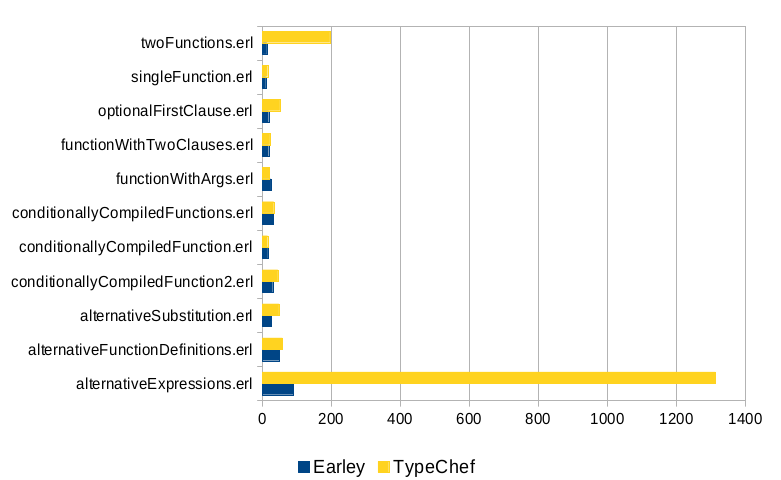
\includegraphics[width=\linewidth]{performance.png}
\caption{Время работы на тестовых данных (мс.)}
\label{chart}
\end{figure}

Из графика \ref{chart} видно, что решения показывают сравнимую скорость работы на большинстве тестов. Медианные значения составляют 25 и 45 миллисекунд для Earley и TypeChef, соответственно.

Тесты, в которых синтаксический анализатор, реализованный с помощью TypeChef, показывает значительно худшие результаты имеют следующее отличие --- в них присутствуют арифмeтические выражения с альтернативными подвыражениями --- один из таких тестов приведен в листинге \ref{altexpr}. 

\begin{minipage}{\linewidth}
\begin{lstlisting}[caption={Один из тестов с альтернативными подвыражениями},language=Erlang,label=altexpr]
-ifdef(X).
-define(EXPR, * 19).
-else.
-define(EXPR, + 18).
-endif.

foo() ->
    (11 ?EXPR) - 94.
\end{lstlisting}
\end{minipage}

Низкая скорость разбора может быть связана с неудачным описанием списочных конструкций, что приводит к экспоненциальной сложности разбора таких выражений в TypeChef.

Из вышеописанного можно заключить, что разработанное решение не уступает TypeChef в производительности, требуя при этом значительно меньших усилий при описании входного языка.

\subsection{Направления развития решения}

В этом подразделе описываются возможные направления работы связанные с улучшением решения, предлагаемого в настоящей работе, и устранением имеющихся в нем недостатков. 

На данный момент библиотека не позволяет использование в грамматике пустых правил. Известны модификации алгоритма Earley, позволяющие обрабатывать пустые правила \cite{emptyrules} --- они могут быть использованы и в модифицированном алгоритме, описанном в подразделе \ref{subsec:earleymodification}.

Выразительность предметно-ориентированного языка для описания грамматик входных языков также может быть увеличена при помощи поддержки EBNF синтаксиса.

Расширение функциональности предметно-ориентированного языка также возможно за счет применения аннотаций к правилам и за счет учета порядка их следования для разрешения неопределенностей при разборе. Это позволило бы описывать, например, грамматику выражений в интуитивно понятной форме, например, так: 

$$Expr\ ::=\ Expr\ +\ Expr\ //left-associative$$.

Модифицированный алгоритм Earley может быть улучшен при помощи обработки некоторых специальных случаев --- таких, например, как списочные структуры в грамматиках языка. На данный момент, наличие во входном тексте списка элементов, элементы которого находятся в различных ветвях условной компиляции, приводит к экспоненциальной от количества альтернативных элементов списка зависимости количества требуемой оперативной памяти и времени восстановления графа синтаксического разбора. Этого можно избежать, допуская не только альтернативное, но и условное вхождение элементов в списочные структуры.

Разработанный алгоритм может быть исследован на наличие возможности поддержания контекстов при разборе ветвей условной компиляции, что позволило бы проводить синтаксический анализ текстов на контекстно-зависимых языках программирования.

Другим возможным направлением работы является разработка предметно-ориентированного языка для описания парсера и интерпретатора инструкций препроцессора --- это позволило бы существенно сократить трудозатраты на разработку синтаксического анализатора исходного кода, содержащего инструкции препроцессора.

\clearpage

\section{Заключение}

Настоящая работа продемонстрировала возможность создания инструмента, позволяющего производить синтаксический анализ исходного кода, содержащего инструкции препроцессора, используя синтаксический анализатор исходного кода языка препроцессора, средства интерпретации его инструкций и грамматику языка программирования.

В работе предложена модификация алгоритма синтаксического анализа Earley, использование которой позволяет восстанавливать синтаксические деревья, соответствующие всем возможным конфигурациям препроцессора.

Предложенный алгоритм был реализован в библиотеке позволяющей создавать синтаксические анализаторы исходного кода, содержащего инструкции препроцессора. Библиотека была применена для синтаксического анализа исходного кода на подмножестве языка Erlang.

Было произведено сравнение разработанной библиотеки с аналогичным решением TypeChef --- разработанное решение позволяет с меньшими трудозатратами реализовать синтаксический анализатор исходного кода, содержащего инструкции препроцессора, обладающий сравнимыми характеристиками производительности.

Использование подхода предложенного в этой работе позволяет существенно сократить время на разработку синтаксического анализатора исходного кода, содержащего инструкции препроцессора.

Полученные результаты могут быть использованы для разработки средств автоматической генерации синтаксических анализаторов для языков программирования, используемых с препроцессором.


\cleardoublepage
\phantomsection
\addcontentsline{toc}{section}{Библиография}
\printbibliography


\end{document}
